
\section{Arquitectura de la solución}
En este apartado continuaremos profundizando en los detalles de la solución propuesta en el apartado \ref{solucion}. Describiremos tanto la arquitectura de la aplicación generadora del código como de la aplicación esqueleto de Android que instanciaremos con la plantilla de un informe DICOM-SR.\par

\subsection{Aplicación Android}
Nuestro objetivo último es disponer de una aplicación Android para una determinada ontología de informe médico,  que facilite al personal clínico la tarea de rellenar los informes de los pacientes siguiendo el estándar DICOM-SR. Por lo tanto el código que generaremos deberá contener todos los componentes de una aplicación Android.\par


\subsubsection{Justificación para desarrollar un aplicación nativa para Android}

En este proyecto generamos una aplicación nativa para Android. Antes de entrar en profundidad a describir la anatomía de una aplicación Android, dedicaremos unas líneas a justificar la decisión de escribir una aplicación nativa para Android en lugar de desarrollar una aplicación genérica en HTML5, o utilizando frameworks como Phonegap \cite{phonegap}, Titanium \cite{titanium} o Corona \cite{corona} para crear una aplicación híbrida, o ya que nuestro generador de código está escrito en Python porque no utilizar Python también en Android mediante el framework Kivy\cite{kivy}.\medskip\par

Comenzaremos por argumentar esta última opción ya que es también la más sencilla de rebatir. Que escribamos el generador de código en un lenguaje no implica que el software generado deba estar escrito en ese mismo lenguaje, de hecho esta disociación es un punto fuerte de la generación de código, como ya explicamos en el apartado \ref{sec:generacion-codigo}.\par 
La utilización de Kivy está justificada cuando queremos hacer una aplicación multiplataforma, para dispositivo móviles y de escritorio, sin necesidad de reescribir del código. Aporta la potencia y simplicidad de Python y está recomendado para el desarrollo de juegos o aplicaciones con gran carga gráfica, ya que en el caso de aplicaciones genéricas la interfaz que crea este framework no es la más apropiada.\par
En nuestro caso, la aplicación final es un formulario,  y una de las premisas que nos hemos marcado es que sea intuitiva y fácil de utilizar, por lo tanto los elementos de la interfaz no deberán sorprender al usuario y la interacción con el usuario debe ser ágil. Como generar código en Python supone el mismo esfuerzo que generarlo en cualquier otro lenguaje y no nos ofrece ventajas adicionales descartamos esta opción.\medskip\par

La siguiente opción sería desarrollar una aplicación en HTLM5.\par
Las ventajas principales que tiene esta opción es la rapidez en el desarrollo y que no es necesario pasar un proceso de validación de la misma. Por otra parte se resiente la velocidad de ejecución y no se tiene acceso a todas las funcionalidades de los teléfono o tabletas para las que se desarrolla.\par 
No vamos a necesitar funcionalidades complejas pero el hecho de que la velocidad de ejecución se reduzca respecto a las aplicaciones nativas empeora la usabilidad y por tanto el índice de aceptación de los usuarios y este si es un punto relevante para nuestro objetivo, por lo tanto también descartamos esta opción.\medskip\par

Finalmente quedaría la opción de desarrollar una aplicación híbrida.\par
Esta opción puede hacer uso de las funcionalidades de las tabletas y puede funcionar a la misma velocidad que una aplicación nativa, además tiene aporta el beneficio de que las aplicaciones sobre estos frameworks son más sencillas de desarrollar, pero aportan las complicaciones propias de instalar y trabajar con el framework.\par
Nuestro objetivo es que con un fichero DICOM-SR se genere de automáticamente una aplicación Android. El esqueleto de la aplicación en Android podemos tenerlo preparado e instanciar la aplicación para el fichero concreto, en cambio incluir un framework introduce un nivel más que nos complica la generación automática. Y respecto a la complicación del desarrollo, como el código que generamos lo hacemos mediante generación automática guiada por modelos, desarrollar una aplicación en Anroid no implica un esfuerzo mucho mayor que hacerlo para algún framework para aplicaciones híbridas.\medskip\par

Por lo tanto la opción que más se adapta a las necesidades concretas de este proyecto es el desarrollo de una aplicación nativa para Android.\par

\subsubsection{Esquema de una aplicación Android}
Las aplicaciones Android las aplicación siguen normalmente el patrón de desarrollo Modelo-Vista-Controlador(MVC).
%, o siendo más específicos el patrón de desarrollo Modelo-Vista-Presentador (MVP) que es una evolución del anterior. 
El modelo y los presentadores o controladores se programan en Java y para definir la interfaz de usuario se utilizan ficheros XML.\par
Una aplicación que sigue este patrón de diseño se compone por:
\begin{itemize}
\item \textbf{Vista}: Contiene la interfaz de usuario y las cadenas de texto para internacionalizar dicha interfaz.\par
\item \textbf{Modelo}: Es la información del sistema, encapsula el estado del sistema. 
\item \textbf{Controlador}: Responde a los eventos generados por la vista y interactua con el modelo. 
\end{itemize}

\begin{figure}[ht]
\centering
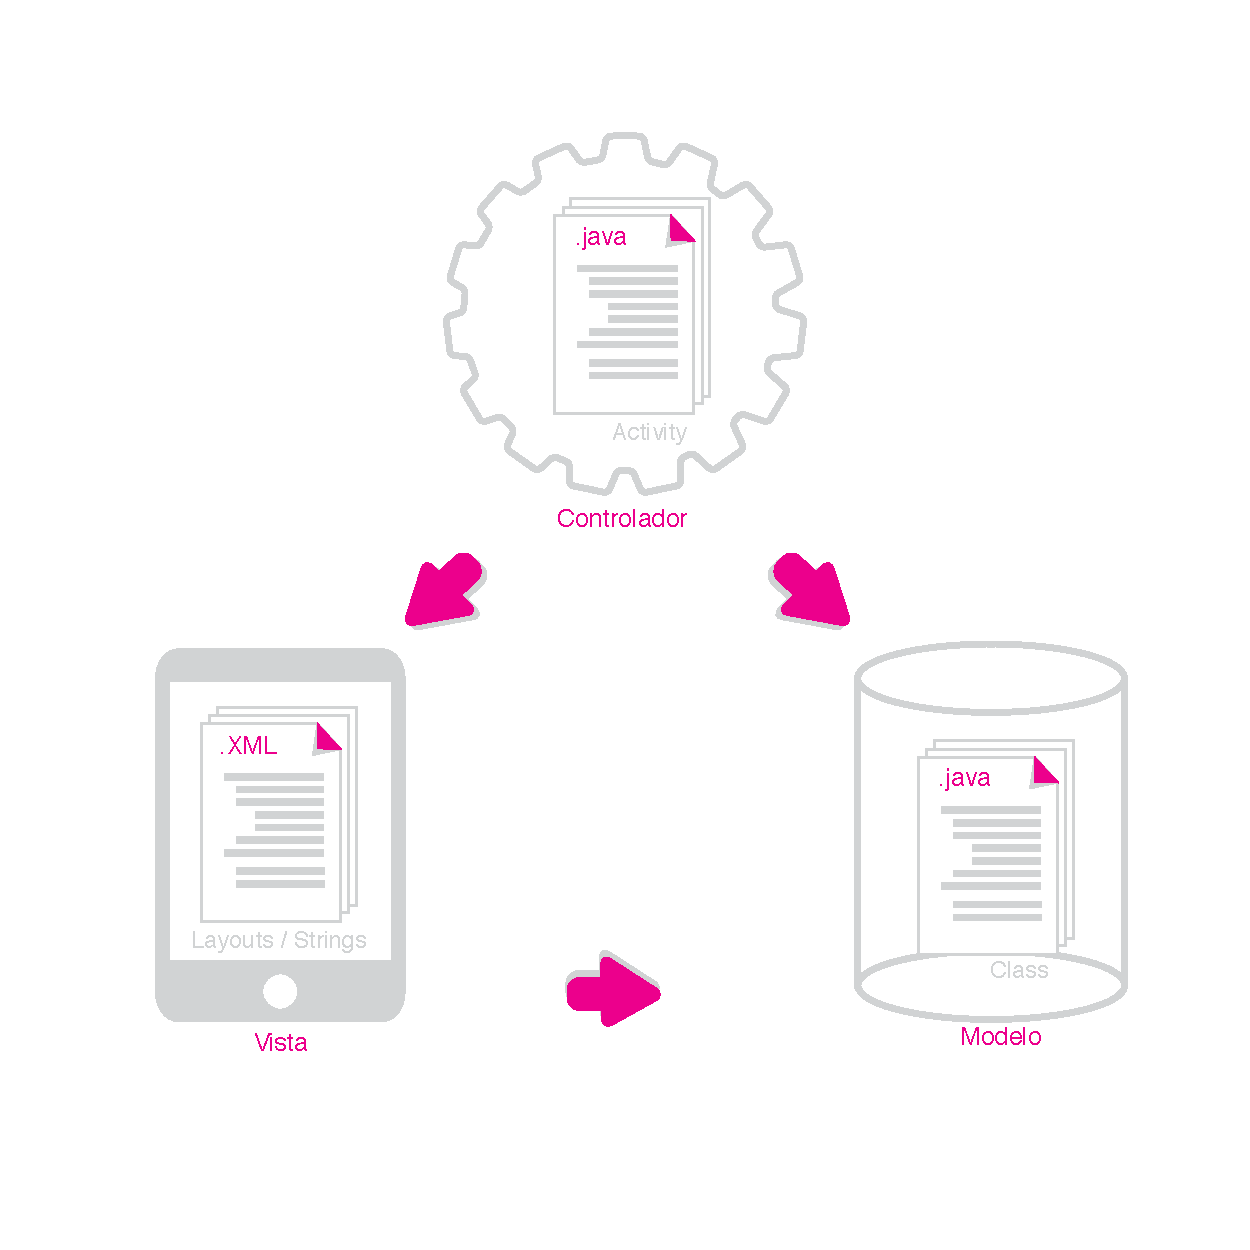
\includegraphics[scale=0.5]{./imgs/esquemas/mvc.pdf}
\caption{Generación parcial de clases}
\label{fig:mvc}
\end{figure}

En la figura \ref{fig:mvc}, vemos el esquema del patrón de desarrollo MVC aplicado en una aplicación Android.\par
Las partes de las que se compone una aplicación Android son las siguientes:
\begin{itemize}
\item \textbf{Vista}: La vista de la aplicación se desarrolla mediante ficheros XML. La vista en Android se compone fundamentalmente por dos elementos: los ficheros XML que definen la interfaz de usuario, que podemos encontrar en \emph{\textbackslash{res}\textbackslash{layout}} y por otra parte tenemos los ficheros XML con las cadenas de texto que se utilizarán en la interfaz, correctamente internacionalizadas y almacenadas en \emph{\textbackslash{res}\textbackslash{values}}. Adicionalmente se puede definir estilos para los elementos de la interfaz gráfica, análogamente a como se hace en CSS, estos ficheros de estilo los podemos encontrar también en \emph{\textbackslash{res}\textbackslash{values}}. Para soportar distintos tipos de pantalla en Android, las imágenes y los estilos se organizan dentro de carpetas determinadas en la aplicación Android y en función de la resolución del dispositivo se cargarán unas u otras.
\item \textbf{Modelo}: El modelo en para una aplicación Android no difiere del modelo en otro lenguaje. Se trata de una serie de clases con la información del sistema. En nuestro caso serán las clases que contengan la información del informe médico. Encapsularemos el modelo dentro del paquete \emph{model}.
\item \textbf{Controlador}: Finalmente los controladores en las aplicaciones Android son las Actividades (\emph{Activity}). Las actividades gestionan la interfaz de usuario, interactuan con el usuario y acceden al modelo bien para mostrarlo en la vista o para modificarlo. 
\end{itemize}

Esta estructura de ficheros de la aplicación Android que nos servirá como framework para instanciar las aplicaciones concretas sobre un informe DICOM-SR y señalando las rutas dónde irán los ficheros que generaremos podemos verla en forma de árbol en la figura \ref{tree:AndroidFramewok}.\par

\begin{figure}

\centering
\framebox[1.05\textwidth]{%
\begin{minipage}{0.95\textwidth}
	\dirtree{%
		.1 \textbf{meer-framework}/.
		.2 {\color{RubineRed} AndroidManifest.xml.}.
		.2 assets/. 
		.3 \vdots.
		.2 bin/. 
		.3 \vdots.
		.2 gen/. 
		.3 \vdots.
		.2 libs/. 
		.3 \vdots.
		.2 \textbf{src}/.
		.3 \textbf{com}/.
		.4 \textbf{i3m}/.
		.5 \textbf{meer}/.
		.6 {\color{RubineRed} *.java }\DTcomment{\emph{Actividades}}.
		.6 \textbf{model}/.
		.7 {\color{RubineRed} *.java }\DTcomment{\emph{Modelo}}.
		.2 \textbf{res}/.
		.3 drawable-hdpi/.
		.4 \vdots\DTcomment{\emph{Iconos e imágenes para alta resolución (> 640dp x 480dp)}}.
		.3 drawable-ldpi/.
		.4 \vdots\DTcomment{\emph{Iconos e imágenes para baja resolución (> 426dp x 320dp)}}.
		.3 drawable-mdpi/.
		.4 \vdots\DTcomment{\emph{Iconos e imágenes para resolución media (> 470dp x 320dp)}}.
		.3 drawable-xhdpi/.
		.4 \vdots\DTcomment{\emph{Iconos e imágenes para extra alta resolución (> 960dp x 720dp)}}.
		.3 layout/.
		.4 {\color{RubineRed} *.xml }\DTcomment{\emph{Vista: UI}}.
		.3 menu/. 
		.4 \vdots\DTcomment{\emph{Vista: menús}}.
		.3 values/. 
		.4 {\color{RubineRed} *.xml }\DTcomment{\emph{Vista: estilos y cadenas de texto}}.
		.3 values-11/. 
		.4 {\color{RubineRed} *.xml }\DTcomment{\emph{Vista: estilos para API 11}}.
		.3 values-14/. 
		.4 {\color{RubineRed} *.xml }\DTcomment{\emph{Vista: estilos para API 14}}.
	}
\end{minipage}
}
\caption{Estructura de ficheros de la aplicación framework Android}
\label{tree:AndroidFramewok}
\end{figure}

\subsection{Aplicación generadora de código}
La aplicación que generará el código a partir de un fichero con una plantilla DICOM-SR está escrita en Python. La aplicación la organizamos siguiendo el esquema de ficheros de una librería de Python, para poder utilizarla en un futuro dentro de en un framework más completo. \par
El código de la aplicación se estructura de manera lógica en función de las tareas a realizar. Las parte más importantes son las siguientes:
\begin{itemize}
\item\emph{Análizador sintáctico}: realiza el análisis sintáctico y almacena la información en una estructura de datos en memoria.
\item\emph{Generador de código}: a partir del informe DICOM-SR cargado en memoria genera el código necesario para instanciar la aplicación Android.
\item\emph{Gestión de la configuración y los ficheros}: lee la configuración del usuario y la aplica en la generación de código.
\item\emph{Modelo del informe}: Estructura de datos que almacena en memoria el informe DICOM-SR.
\end{itemize}
Estas secciones lógicas las encontraremos en el código de la aplicación como aparecen en la figura \ref{tree:meer}.\par
Para llamar al generador de código, \emph{fromDicomAndroid.py}, y generar los ficheros necesarios para crear una aplicación Android, lo ejecutaremos pasando como parámetros el fichero con la plantilla DICOM-SR y el método de internacionalización empleado. Vemos un ejemplo de como se lanzará el generador de código en el segmento de código \ref{fromDicomAndroid}.
\begin{lstlisting}[language=bash,label=fromDicomAndroid,caption=Ejecución del generador de código]
	./fromDicomtoAndroid.py ../../res/xml/02_Mamography_Unix.xml i18n    
\end{lstlisting}


\begin{figure}
\centering
\framebox[1.05\textwidth]{%
\begin{minipage}{0.95\textwidth}
	\dirtree{%
		.1 \textbf{meer}/.
		.2 \textbf{core}/ \DTcomment{\emph{Gestión de la configuración y Estructuras de datos}}.
		.3 config.py \DTcomment{\emph{Funciones que gestionan la configuración}}.
		.3 config\_variables.py \DTcomment{\emph{Cadenas de los ficheros de configuración.}}.
		.3 container.py \DTcomment{\emph{Estructura de datos que modela un contenedor}}.
		.3 dicom.py \DTcomment{\emph{Estructura de datos del informe}}.
		.3 dicomSR.py \DTcomment{\emph{Árbol con el informe DICOM}}.
		.3 files.py \DTcomment{\emph{Gestión de los ficheros generados}}.
		.3 tree.py \DTcomment{\emph{Árbol estándar}}.
		.3 types.py \DTcomment{\emph{Estructuras de datos de los tipos del informe}}.
		.2 \textbf{parser}/ .
		.3 handler.py \DTcomment{\emph{Analizador sintáctico}}.
		.2 \textbf{settings}/ \DTcomment{\emph{Ficheros de configuración}}.
		.3 \textbf{ontologies} \DTcomment{\emph{Configuración basada en la ontología}}.
		.4 4.ini .
		.4 5.ini.
		.4 \vdots.
		.3 output\_paths.ini \DTcomment{\emph{Ruta para los ficheros generados (Usuario)}}.
		.3 settings.ini \DTcomment{\emph{Configuración del sistema (Defecto)}}.
		.2 \textbf{templates/} \DTcomment{\emph{Plantillas y generador de código}}.
		.3 \textbf{activities/} \DTcomment{\emph{Plantillas de actividades y AndroidManifest}}.
		.4 \vdots.
		.3 \textbf{layouts/} \DTcomment{\emph{Plantillas de la interfaz de usuario }}.
		.4 \vdots.
		.3 \textbf{model/} \DTcomment{\emph{Plantillas del modelo de clases}}.
		.4 \vdots.
		.3 \textbf{properties/} \DTcomment{\emph{Ficheros de internacionalización}}.
		.4 \vdots.
		.3 \textbf{strings/} \DTcomment{\emph{Plantillas de internacionalización}}.
		.4 \vdots.
		.3 activities\_handler.py  \DTcomment{\emph{Generador de las actividades}}.
		.3 handler.py  \DTcomment{\emph{Generador de código}}.
		.3 layouts\_handler.py  \DTcomment{\emph{Generador de la IU}}.
		.3 model\_handler.py  \DTcomment{\emph{Generador del modelo}}.
		.3 string\_handler.py  \DTcomment{\emph{Generador de la internacionalización}}.
		.2 {\color{RubineRed} fromDicomAndroid.py} \DTcomment{\emph{Script que genera el código Android}}.
		.2 requirements.txt.\DTcomment{\emph{Requerimientos de la aplicación}}.
	}
\end{minipage}
}
\caption{Estructura de ficheros de la aplicación Python generadora de código}
\label{tree:meer}
\end{figure}
\subsubsection{Diagrama de clases}
A continuación veremos los diagramas de clases de las secciones más relevantes del código.\par
El código que gestiona la configuración y el generador de código agrupan un conjunto de funciones y veremos su implementación en los apartados \ref{sec:configuracion} y \ref{sec:generacion} respectivamente.\par
Comenzaremos por ver en la figura \ref{fig:uml-parser}, la clase creada para realizar el análisis sintáctico, extiende de \emph{xml.sax.handler.ContentHandler}, que es el módulo de la librería estándar de Python que implementa la API simple de XML en Python obviamente. \par

\begin{figure}[ht]
\centering
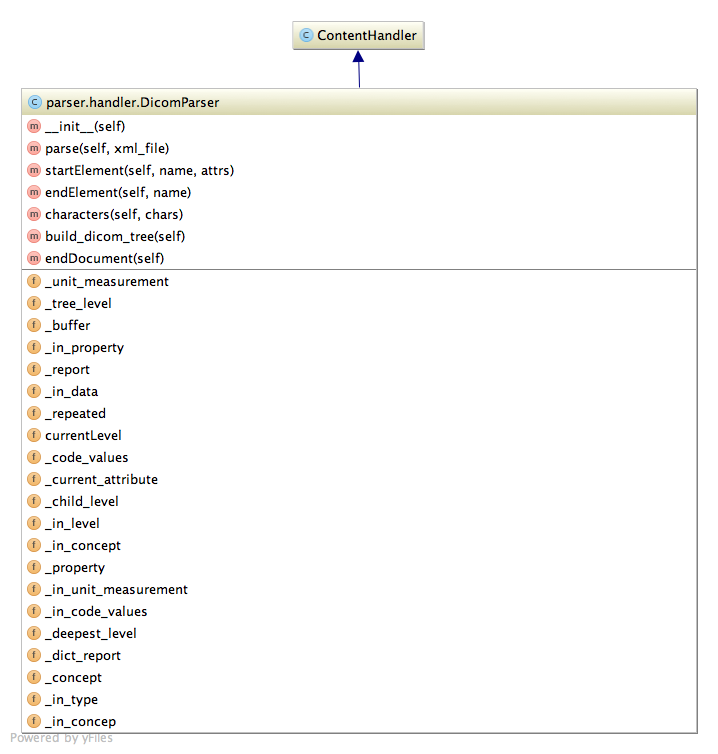
\includegraphics[scale=0.6]{./imgs/diagramasUML/parser.png}
\caption{Diagrama de clase UML del analizador sintáctico.}
\label{fig:uml-parser}
\end{figure}

Al emplear un analizador de tipo SAX, necesitaremos una estructura de datos que a medida que leemos el fichero DICOM-SR almacene la información del mismo. La figura \ref{fig:uml-dicom} muestra el diagrama de esta clase. Por simplicidad el informe se modela mediante una lista de contenedores con la información del contenedor DICOM. Cada contenedor guarda información acerca de que contenedor es su padre. \par

\begin{figure}[ht]
\centering
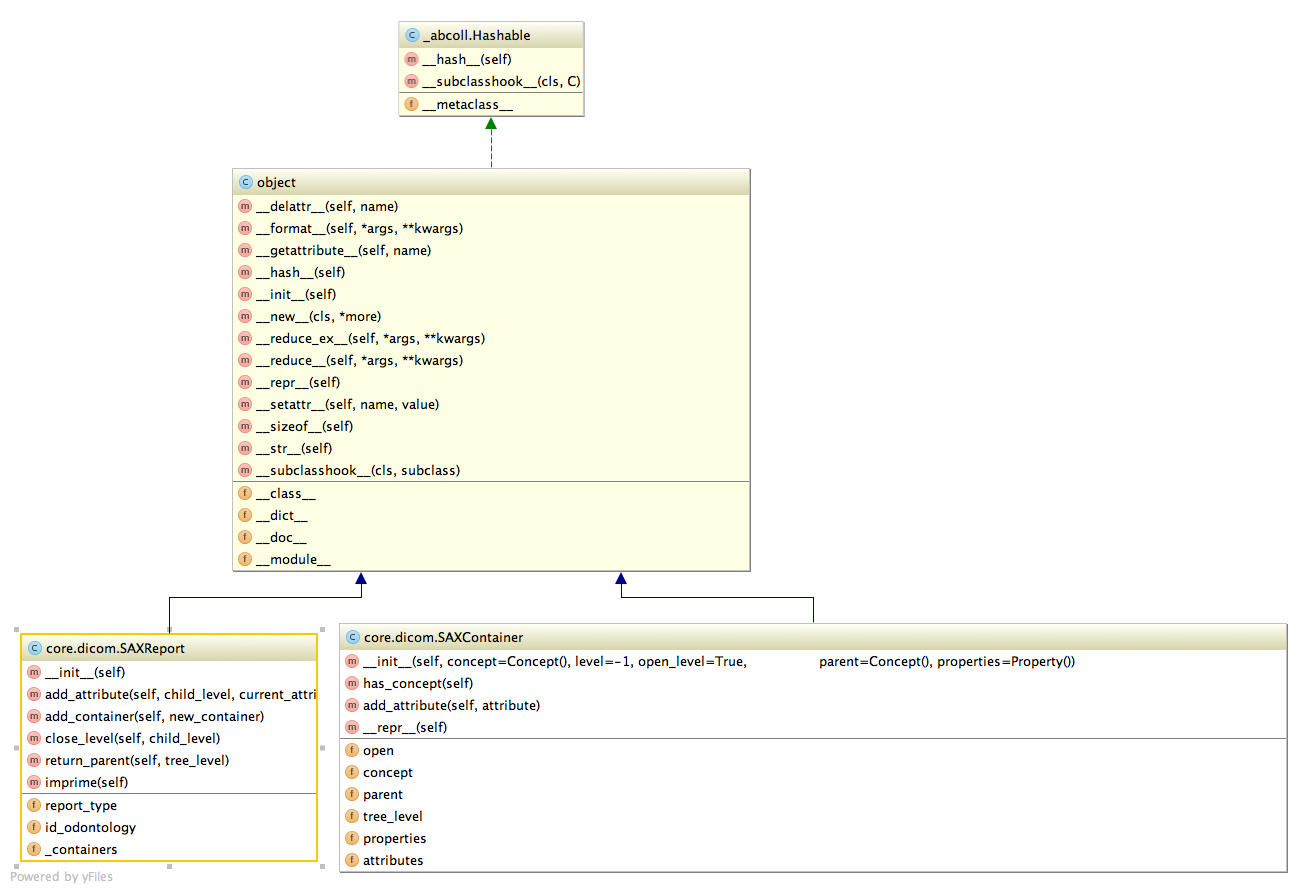
\includegraphics[scale=0.35]{./imgs/diagramasUML/core/dicom.png}
\caption{Diagrama de clase UML de la estructura de datos del informe DICOM.}
\label{fig:uml-dicom}
\end{figure}

Una vez terminado el análisis sintáctico, tener el informe como una lista de contenedores ralentiza el proceso de extraer información para generar el informe, así que guardamos la información dentro de un árbol.\par
Para esto disponemos de una clase árbol genérica que podemos ver en el diagrama \ref{fig:uml-tree}. Los nodos de este árbol estarán formados por contenedores con la información de un contenedor de tipo DICOM. El diagrama UML que corresponde a estos contenedores es el de la figura \ref{fig:uml-container}. Todo el informe se encapsula dentro de la clase DicomSR y podemos ver el diagrama de esta clase en la figura \ref{fig:uml-dicomSR}.\medskip \par

Terminamos esta sección con el diagrama UML de los tipos de datos soportados en DICOM-SR. Dentro de los contenedores, almacenamos conceptos DICOM, y son estos conceptos los que se modelan en el diagrama de la figura \ref{fig:uml-types}.
\begin{figure}[ht]
\centering
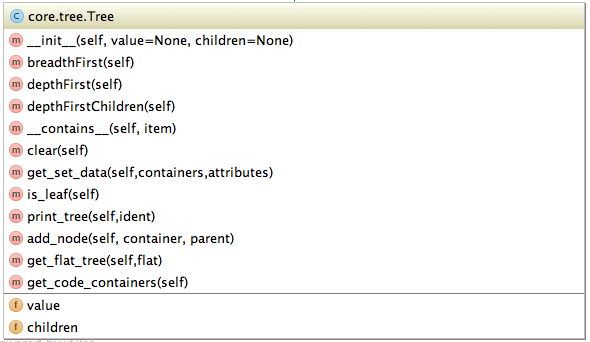
\includegraphics[scale=0.5]{./imgs/diagramasUML/core/tree.png}
\caption{Diagrama de clase UML del árbol genérico}
\label{fig:uml-tree}
\end{figure}

\begin{figure}[ht]
\centering
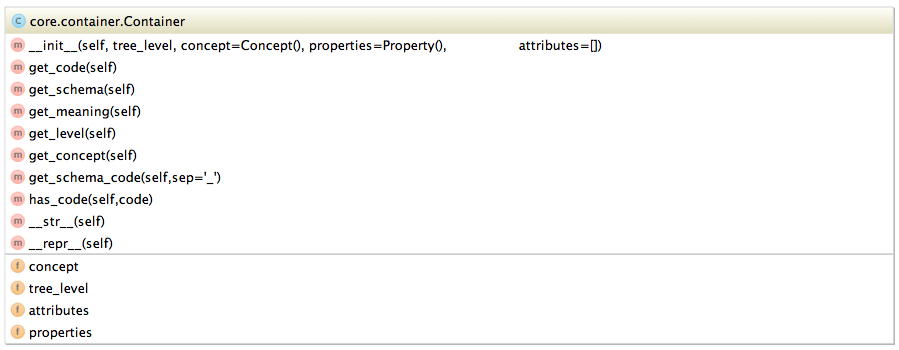
\includegraphics[scale=0.5]{./imgs/diagramasUML/core/container.png}
\caption{Diagrama de clase UML del contenedor DICOM}
\label{fig:uml-container}
\end{figure}

\begin{figure}[ht]
\centering
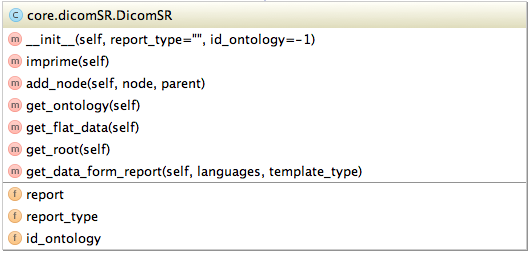
\includegraphics[scale=0.5]{./imgs/diagramasUML/core/dicomSR.png}
\caption{Diagrama de clase UML de la estructura de datos del informe DICOM utilizando un árbol.}
\label{fig:uml-dicomSR}
\end{figure}

\begin{figure}[ht]
\centering
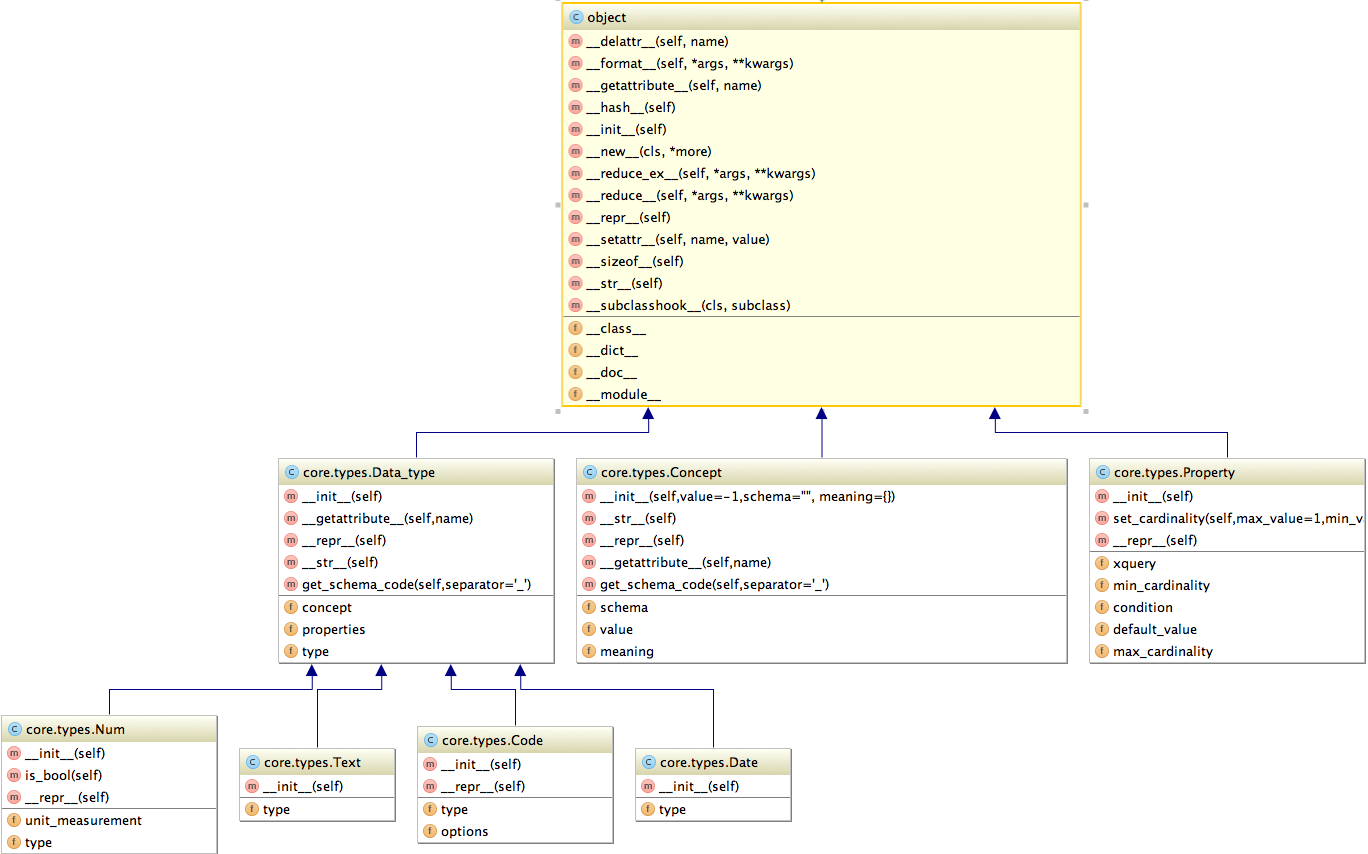
\includegraphics[scale=0.35]{./imgs/diagramasUML/core/types.png}
\caption{Diagrama de clase UML de los conceptos DICOM.}
\label{fig:uml-types}
\end{figure}


\section{Diseño de la experiencia de usuario}
En el apartado \ref{sec:UI} ya hemos hablado de el impacto que tiene el diseño de las interfaces que realicemos en la aceptación de las aplicaciones por parte de los usuarios.\par
Para que la aplicación Android que generermos automáticamente sea gráficamente atractiva para los usuarios finales, deberemos diseñar correctamente toda la experiencia de usuario.\par
En la industria actual se intenta involucrar a todos los responsables de un desarrollo para lograr que la experiencia del usuario sea satisfactoria. Al tratarse de un proyecto personal trataremos, en la medida de lo posible, de asumir todos los roles que entran en juego al diseñar una experiencia de usuario.\par
En el esquema de la figura \ref{fig:uxui} podemos ver los roles que intervienen en el diseño de una experiencia de usuario satisfactoria.\medskip\par

\begin{figure}[ht]
\centering
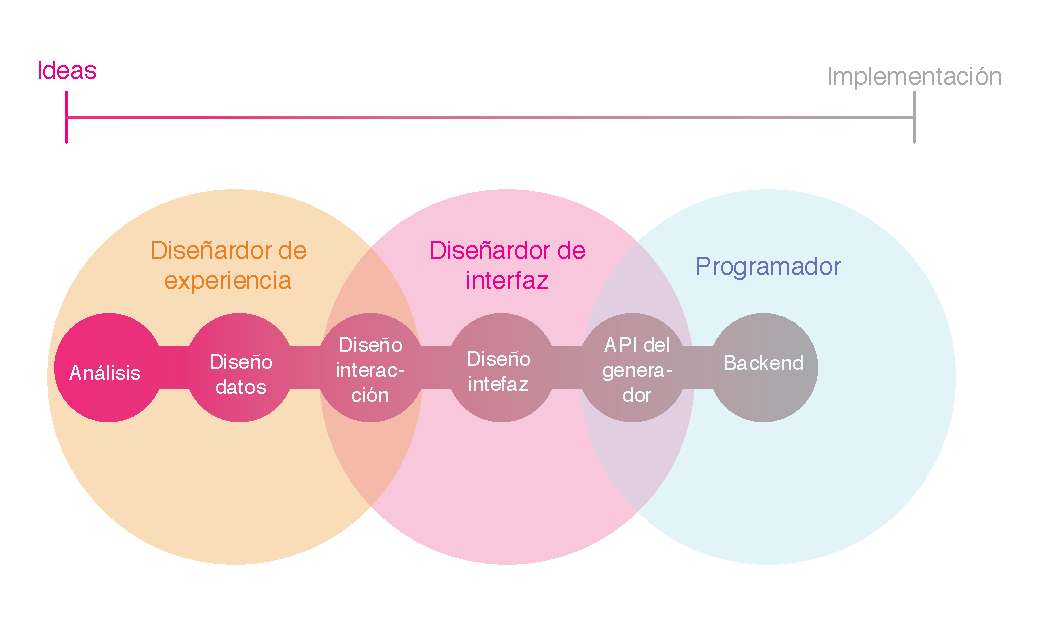
\includegraphics[scale=0.7]{./imgs/esquemas/uxui.pdf}
\caption{Roles que intervienen en el desarrollo de aplicaciones útiles}
\label{fig:uxui}
\end{figure}

Para diseñar la experiencia de usuario debemos analizar el problema desde el punto de vista del usuario, pensar el uso que el usuario hará de la herramienta que vamos a crear y como se integrará en su rutina. Analizamos el trabajo facultativo, así como los datos que debe contener un informe médico estructurado, a partir de estos datos diseñaremos la interacciones que realizará el usuario con la aplicación.\par
Después de varias iteraciones con los prototipos llegamos a la conclusión de que la forma más coherente y genérica de estructurar la aplicación es que cada pantalla corresponda a los datos de un nivel del informe estructurado. Además en cada una de estas pantallas el usuario podrá acceder a un resumen del informe que esta introduciendo, así como la posibilidad de navegar entre niveles de manera intuitiva y acceder a validar la información en cualquier momento.Podemos ver la primera iteración del diseño de la experiencia en el apartado \ref{sec:ui-mockup}.\medskip\par

Simultáneamente al diseño de la interacción, diseñaremos la interfaz de usuario.\par
Veremos en el apartado \ref{sec:estilo}, la guía de estilo que hemos definido para este proyecto.\par

\subsection{Guía de estilo}\label{sec:estilo}

Android es muy versátil en lo que a desarrollo de interfaz de usuario se refiere, lo cual es algo positivo pero que si no se diseña con cuidado la interfaz pude dar lugar a aplicaciones inconsistentes desde el punto de vista del diseño. Para incentivar el diseño correcto de aplicaciones, Android tiene una guía exhaustiva de diseño de interfaces para sus dispositivos \cite{android:design} que en este proyecto seguiremos. \par

Debido a la naturaleza de la aplicación y que uno de nuestros objetivos es que la aplicación sea rápida y simple de utilizar, prescindiremos de las imágenes en la medida de lo posible. Todo el peso del diseño recaerá en la tipografía, el esquema de color y la estructura interna que organiza estos elementos, es decir, la cuadrícula.\par
\subsubsection{El sistema de cuadrícula}
Aunque el diseño de interfaces utilizando la cuadrícula es un método que nos pueda parecer actual, se trata de un sistema desarrollado después de la segunda guerra mundial y que se integra en el diseño internacional o diseño suizo.\par
Se trata simplemente de un diseño en el que una cuadrícula organiza los elementos del diseño, en nuestro caso de la interfaz de usuario. Entre los principales puntos fuertes que tiene este sistema es que ayuda a la navegación, capta la atención del usuario facilitando la lectura y escritura y son diseños estables y previsibles lo que hace que sea más sencillo a los usuarios interactuar con estos diseños.\par
En la figura \ref{fig:grid}, vemos un ejemplo de la cuadrícula superpuesta sobre una de las pantallas de la interfaz del prototipo. 

\begin{figure}[ht]
\centering
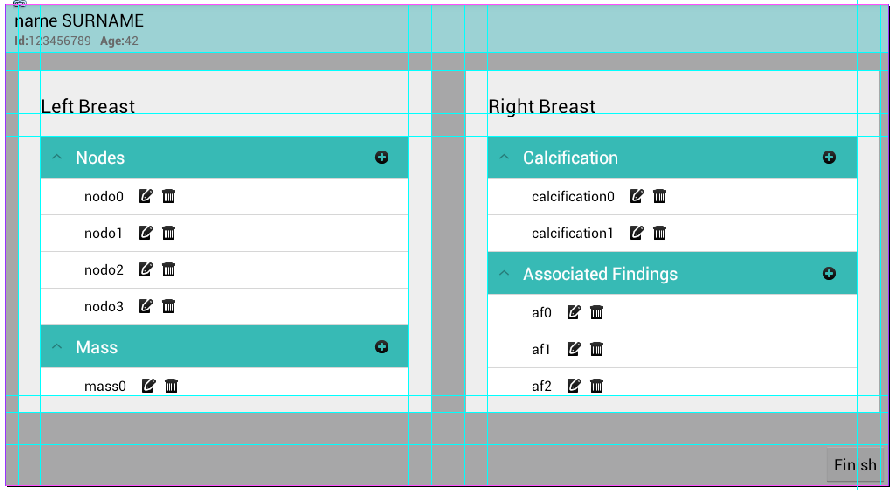
\includegraphics[scale=0.5]{./imgs/ui/grid.png}
\caption{Sistema de cuadrícula}
\label{fig:grid}
\end{figure}

\subsubsection{La tipografía}
Con la versión 3.2 de Android se introduce \emph{Roboto}, una tipografía de palo seco diseñada específicamente para dar respuesta a los requisitos de los dispositivos con alta resolución de pantalla.\par
Se trata una tipografía que favorece la lectura en dispositivos digitales por no tener remates, porque la mancha está balanceada y los ojos de los caracteres son amplios.\par

\subsubsection{El esquema de color}
Finalmente hablaremos del esquema de color escogido para la aplicación.\par
Aunque lo general para las aplicaciones dentro del ámbito médico es emplear colores fríos en los que predominan los azules y los verdes, porque se trata de colores que sugieren espacios asépticos y  tranquilos.\par
Empleamos turquesas y grises en la paleta básica y utilizamos como color secundario dos tonos naranjas. La paleta tiene una componente cálida que se aleja de las recomendaciones, pero que confiere a la aplicación un carácter más orgánico, lo que suele aumentar el nivel de aceptación de los usuarios.\par
Se evitan los grandes contrastes, evitando los blancos y los negros puros en la interfaz, lo que reduce la fatiga visual.\medskip\par
Android permite definir paletas de colores como un elemento de los recursos más. La paleta que definimos para la aplicación es la que vemos en el fragmento de código \ref{palette}.

\lstset{escapechar=@,style=dicom}
\begin{lstlisting}[label=palette,caption=Esquema de color]

<?xml version="1.0" encoding="utf-8"?>
<resources>
    <color name="dirtyWhite">#F6F8F8</color>
    <color name="turquoise">#50BAB5</color>
    <color name="babyBlue">#A2D2D5</color>
    <color name="orange">#EB6E51</color>
    <color name="dust">#DDC0B2</color>
    <color name="darkGrey">#686868</color>
    <color name="lightGrey">#A7A7A8</color> 
    <color name="black">#000000</color>
 </resources>

\end{lstlisting}
En la figura \ref{fig:estilo} encontramos un resumen de las características del estilo de la aplicación.\par


\begin{figure}[ht]
\centering
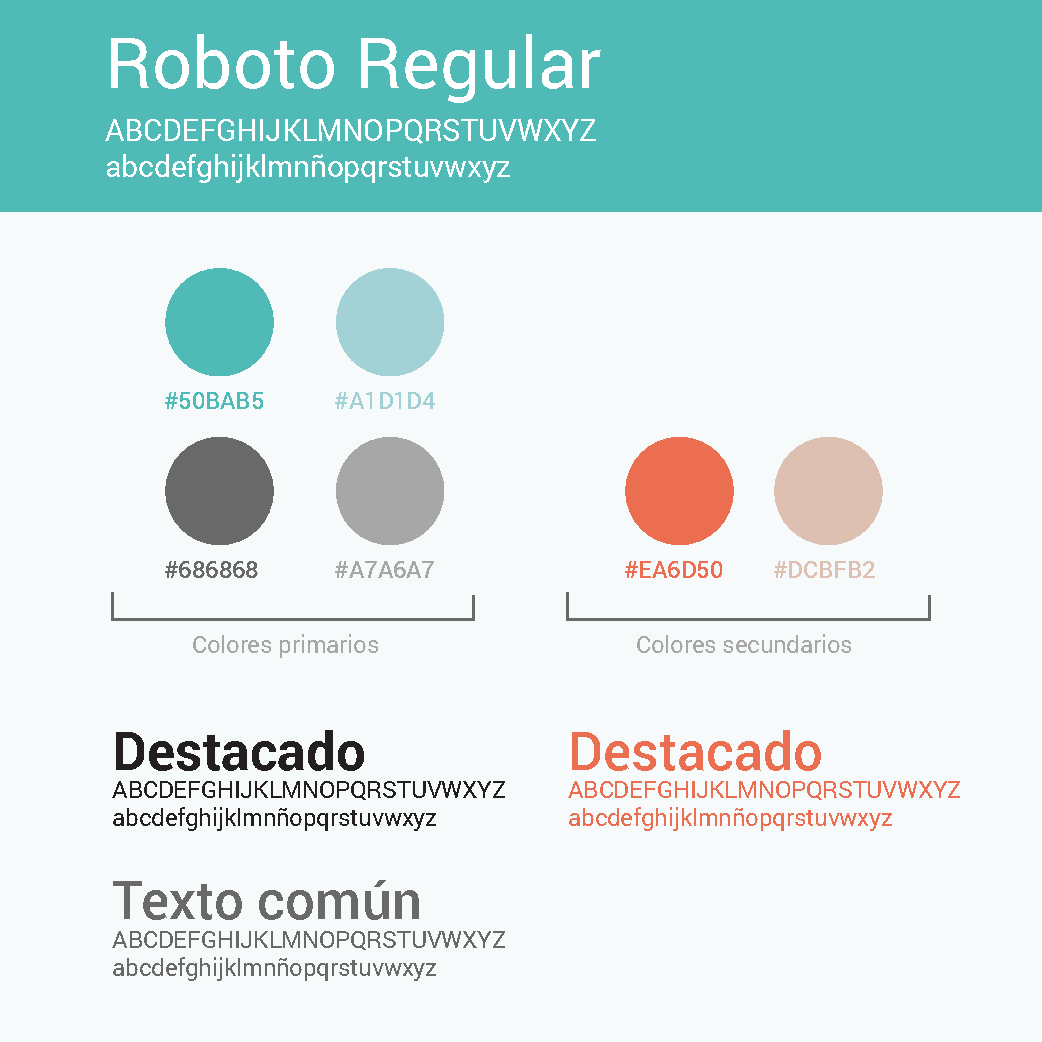
\includegraphics[scale=0.7]{./imgs/ui/estilo.pdf}
\caption{Guía de estilo}
\label{fig:estilo}
\end{figure}

\subsection{Diseño de las interacciones}\label{sec:ui-mockup}
Para diseñar correctamente las interacciones necesitamos conocer  el uso que le dará  el usuario.\par
Si realizáramos el diseño para un informe general no seríamos capaces de captar las necesidades del usuario. Por lo tanto tomamos como ejemplo una mamografía y planteamos las interacciones que el usuario deberá llevar a cabo para introducir el informe de una mamografía.\par
Los bocetos que veremos de estos diseños no siguen las guías de estilo que definimos en el apartado \ref{sec:estilo} porque lo que se pretende validar en este punto es la interacción no la interfaz, de modo que se aísla el diseño de la interfaz de usuario del diseño de las interacciones.\medskip\par
Comenzaremos por la pantalla de inicio que podemos ver en la figura \ref{fig:mockup:ini}. En la parte superior, siempre visible tendemos los datos del paciente para que el facultativo en todo momento sepa fácilmente de quien es el informe que está rellenando.\par

\begin{figure}[ht]
\centering
\includegraphics[page=4,scale=0.4]{./imgs/mockup/mockup.pdf}
\caption{Mockup: Inicio de la aplicación}
\label{fig:mockup:ini}
\end{figure}

También en la parte superior encontramos un menú que al desplegarlo nos permite ver un resumen del informe que se está codificando, en la imagen \ref{fig:mockup:resumen} vemos esta funcionalidad, de este modo el facultativos puede comprobar en todo momento los datos ya introducidos.\par 

\begin{figure}[ht]
\centering
\includegraphics[page=13,scale=0.4]{./imgs/mockup/mockup.pdf}
\caption{Mockup: Barra lateral con el resumen del informe}
\label{fig:mockup:resumen}
\end{figure}

En la parte inferior tendremos dos botones par validar y finalizer el informe. Al inicio estará habilitado el botón de \emph{validar}, y cuando el usuario introduzca datos podrá validar el informe y tras la validación se habilitará el botón para finalizar que creará un informe DICOM con los datos del estudio introducidos.\par
En los dos fragmentos definidos por la cuadricula estructuraremos la información que será diferente para cada nivel del informe médico.\medskip\par
Un flujo de trabajo normal comenzaría como se muestra en la figura \ref{fig:mockup:ini}. A la izquierda vemos los datos que se deben introducir en el nivel superior (identificador del paciente, identificador del estudio,\ldots) y a la derecha veremos un resumen de las lesiones de la mamografía ya codificadas. Como estamos en el inicio y el usuario no ha introducido lesiones, este resumen está vacío.\par
Para codificar una nueva lesión simplemente deberá pulsar en el botón con el texto \emph{Añadir Lesiones}.\medskip\par

Esta acción llevará al usuario a una pantalla similar a la que vemos en la figura \ref{fig:mockup:tree}, donde vemos una lista de las lesiones que puede contener un informe de tipo mamografía. Como hay dos órganos que se estudian en este informe, las anomalías de cada órgano se organizan dentro de una cuadrícula.\par
Al lado de cada elemento del listado hay un icono para añadir una nueva lesión de este tipo. Cuando el usuario pulse sobre un icono para añadir por ejemplo una desectructuración en la mama derecha, la aplicación le llevará hasta un pantalla similar a la que podemos ver en la figura \ref{fig:mockup:add}.\medskip \par

\begin{figure}[ht]
\centering
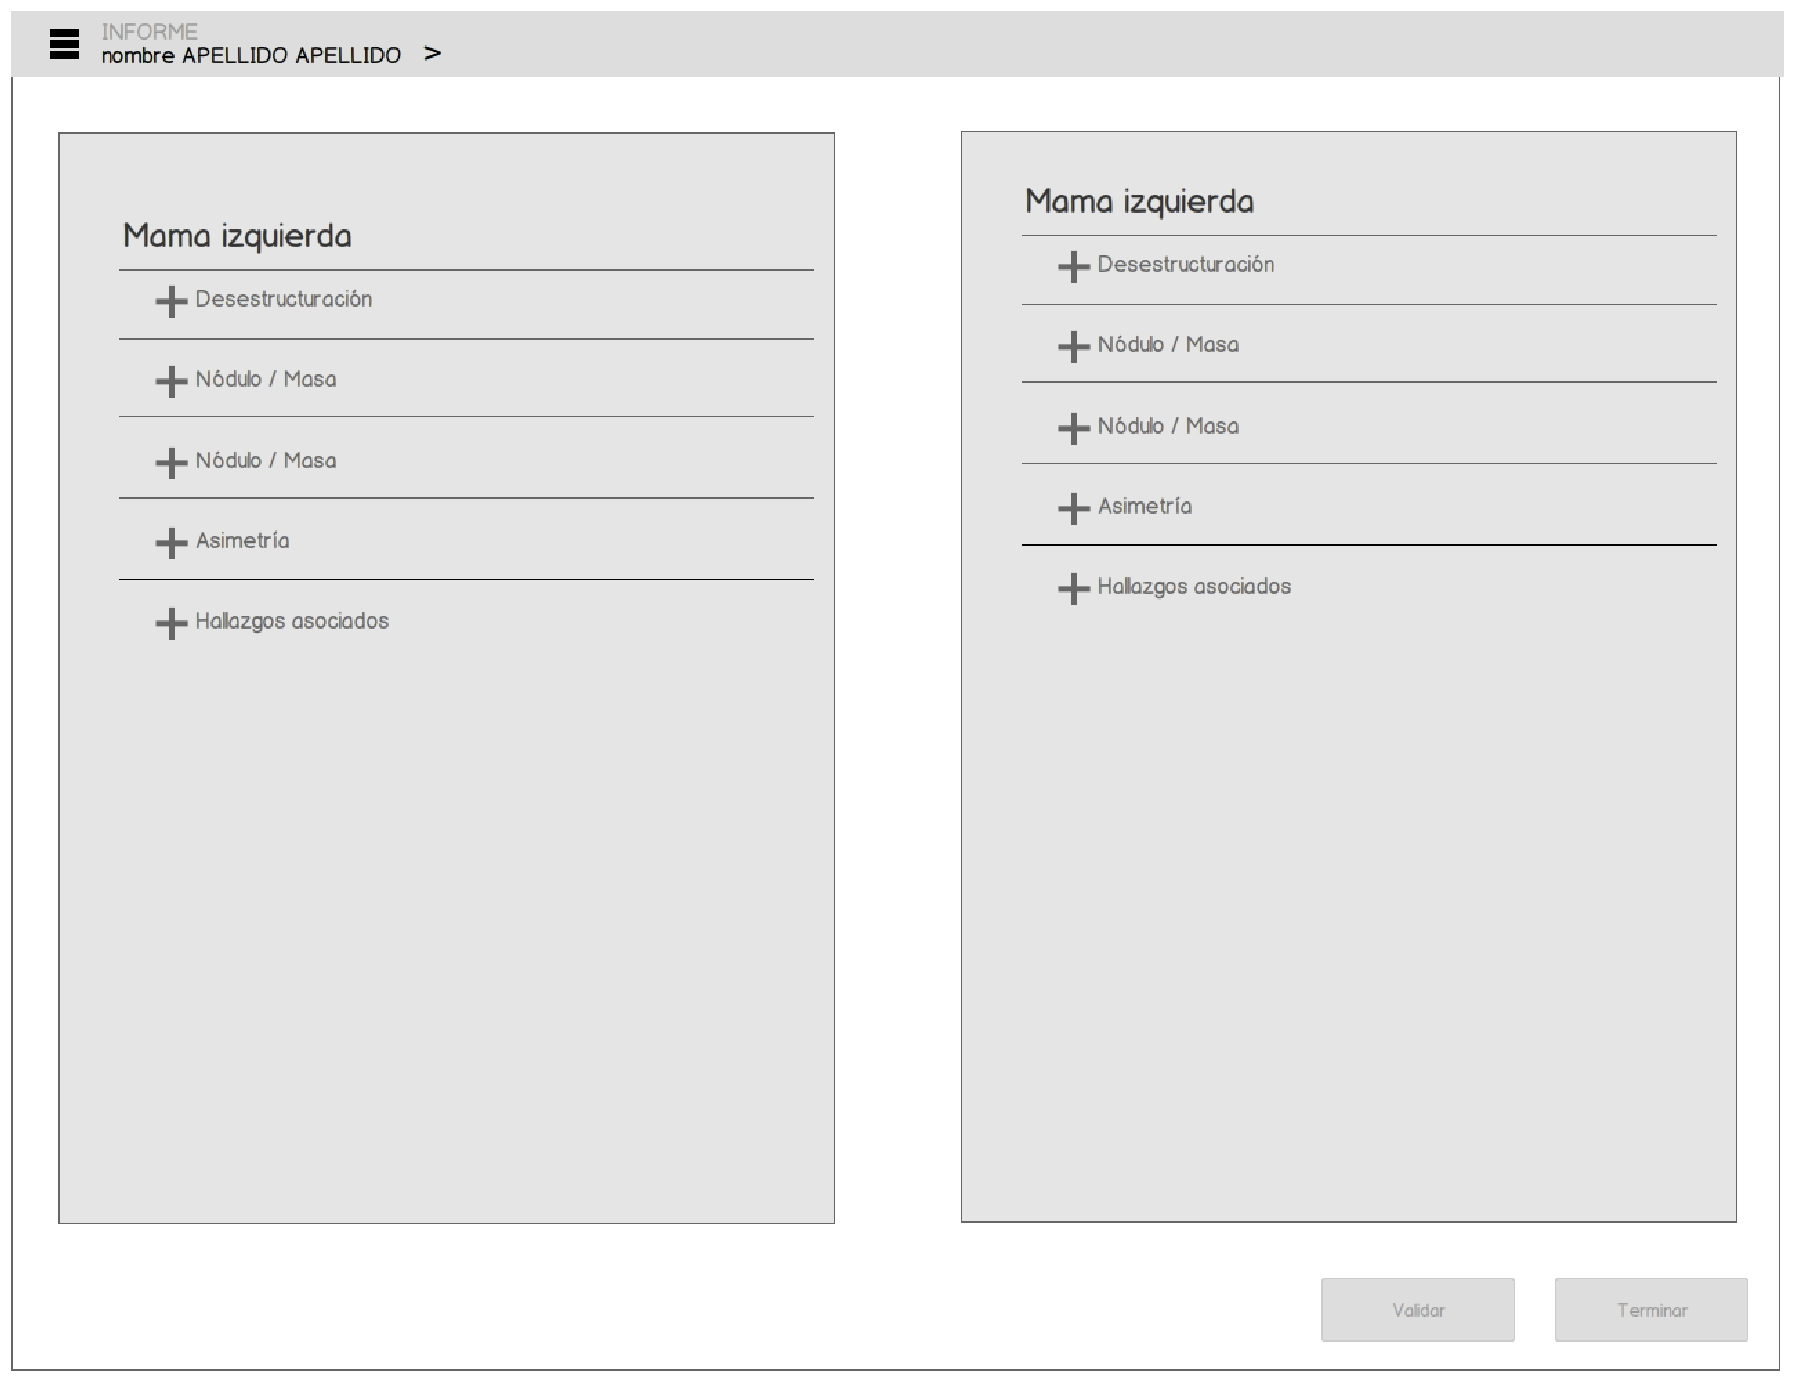
\includegraphics[page=1,scale=0.4]{./imgs/mockup/mockup.pdf}
\caption{Mockup: Lista con las posibles lesiones de una mamografía}
\label{fig:mockup:tree}
\end{figure}

En esta figura vemos que las dos cuadrículas albergan los atributos que definen una desestructuración. El personal clínico llenará estos campos con los datos de un informe concreto y cuando haya terminado de introducir los datos podrá guardarlos, validarlos y descartarlos.\par
Permitimos que la validación se pueda realizar en todos los niveles del informe, facilitando el uso de la aplicación a los usuarios.\medskip\par
Tras introducir unas cuantas lesiones, el usuario las verá en el árbol que contiene las lesiones para cada órgano, agrupadas por el tipo de lesión, como podemos ver en la figura \ref{fig:mockup:treenodes}.\medskip\par

\begin{figure}[ht]
\centering
\includegraphics[page=11,scale=0.4]{./imgs/mockup/mockup.pdf}
\caption{Mockup: Añadir una desestructuración en la mama derecha}
\label{fig:mockup:add}
\end{figure}

Al lado de cada lesión vemos un pequeño icono que abrirá una lista desplegable con las acciones que podemos realizar sobre esa lesión en concreto. De este modo la lista de lesiones se mantiene lo más compacta posible, y sigue siendo fácil realizar acciones sobre una lesión en concreto.\par
También podemos ver en esta imagen que estamos comentando que si la cardinalidad de un tipo de lesión está completa desaparece el icono para incluir nuevas lesiones no permitiendo añadir nuevas lesiones de este tipo.\par
Al pulsar sobre el icono situado a la derecha de la lesión se despliegan las acciones disponibles. Como podemos ver en la figura \ref{fig:mockup:expandable}, las acciones disponibles en este caso son: editar la lesión y eliminarla. Si el usuario decide borrar una lesión verá un mensaje de error como el que se muestra en la figura \ref{fig:mockup:delete}\medskip\par

\begin{figure}[ht]
\centering
\includegraphics[page=5,scale=0.4]{./imgs/mockup/mockup.pdf}
\caption{Mockup: Lista con las lesiones de una mamografía}
\label{fig:mockup:treenodes}
\end{figure}

\begin{figure}[ht]
\centering
\includegraphics[page=7,scale=0.4]{./imgs/mockup/mockup.pdf}
\caption{Mockup: Acciones que un usuario puede realizar sobre una lesión en concreto.}
\label{fig:mockup:expandable}
\end{figure}

\begin{figure}[ht]
\centering
\includegraphics[page=8,scale=0.4]{./imgs/mockup/mockup.pdf}
\caption{Mockup: Aviso de que el usuario va a borrar una lesión.}
\label{fig:mockup:delete}
\end{figure}

Pongámonos en el caso ahora de que el usuario quiere editar una lesión, la aplicación le redirigiría a una pantalla como la que muestra la figura \ref{fig:mockup:edit} con los datos de la lesión a modificar.\par
Si por algun motivo, el usuario deseara volver atrás sin guardar los cambios vería un mensaje advirtiéndolo que los cambios que ha realizado en la lesión, si los hubiera, no se guardarán, como podemos ver en la figura \ref{fig:mockup:warning}.\par

\begin{figure}[ht]
\centering
\includegraphics[page=10,scale=0.4]{./imgs/mockup/mockup.pdf}
\caption{Mockup: Editar una lesión}
\label{fig:mockup:edit}
\end{figure}


\begin{figure}[ht]
\centering
\includegraphics[page=12,scale=0.4]{./imgs/mockup/mockup.pdf}
\caption{Mockup: Aviso de que no se guardan los cambios}
\label{fig:mockup:warning}
\end{figure}


\begin{figure}[ht]
    \centering
        \begin{subfigure}[b]{0.5\textwidth}
                \centering
                \includegraphics[page=2,scale=0.25]{./imgs/mockup/mockup.pdf}
                \caption{Informe pendiente de validar}
                \label{fig:mockup:validated}
        \end{subfigure}%
        ~ 
        \begin{subfigure}[b]{0.5\textwidth}
                \centering
                \includegraphics[page=3,scale=0.25]{./imgs/mockup/mockup.pdf}
                \caption{Informe listo para guardar}
                \label{fig:mockup:finish}
        \end{subfigure}
    \caption{Informe con datos}\label{fig:end}
\end{figure}

Con todo este proceso creamos un documento con las interacciones. Tras validar las interacciones con los usuarios podremos pasar a la siguiente fase del desarrollo de la aplicación.\par

\clearpage
\section{Prototipo}\label{prototipo}

Antes de adentrarnos en la aplicación generadora de código debemos validar que las interacciones y la interfaz de usuario que hemos diseñado y validado, sea correcta dentro del entorno de producción. Para esto, crearemos un prototipo, con parte de la funcionalidad ya implementada de la aplicación Android final.\par

Este prototipo además nos servirá como entrono de pruebas para generar las plantillas de código.\medskip\par

Hemos desarrollado una aplicación para Android que permitiría introducir datos de un informe de tipo \emph{Exploración de Mama}.\medskip\par

El flujo de trabajo es similar al que hemos descrito en el apartado \ref{sec:ui-mockup}.\par
En la figura \ref{fig:prototipo:inicio} vemos la interfaz de incio de la aplicación.\par
Cuando el facultativo vaya a añadir una lesión verá la pantalla mostrada en la figura \ref{fig:prototipo:tree}, donde encontramos todas las posibles lesiones que se pueden asociar a cada órgano.\par 
En este punto el usuario puede seleccionar un tipo de lesión a incluir en el informe y para introducir los datos de esta lesión deberá hacerlo rellenando un formulario como el que vemos en la figura \ref{fig:prototipo:add}. \par
Cuando el informe ya disponga de lesiones podrá ver un listado de las lesiones introducidas agrupadas por tipología como se puede ver en la figura \ref{fig:prototipo:treenodes}. En este punto hay un pequeño cambio respecto al diseño de las interacciones donde las acciones disponibles para cada lesión, editar y borrar, se mostraban en un desplegable. Cuando desarrollamos este prototipo nos dimos cuenta que los pictogramas de las accones eran fácilmente identificables y que al ocultar las acciones en un nivel de anidamiento más algunos usuarios no sabían muy bien como editar o borrar una lesión puesto que estas acciones estaban ocultas. De modo que ahora las acciones se sitúan justo a la derecha del identificador de la lesión.\par
Si el usuario edita una lesión lo haría mediante una pantalla como la que vemos en la figura \ref{fig:prototipo:edit}.\par
Al igual que en el diseño de interfaces propuesto, la banda superior permite tener presente en todo momento al paciente al que pertenece el estudio que se está introduciendo y la banda inferior  encontramos un botón que permite terminar de introducir el informe y obtenerlo en formato DICOM-SR. En lugar de obligar al usuario a validar para después finalizar, simplificamos el proceso uniendo las dos tareas en una única. Cuando el usuario desee terminar de introducir datos y pulse el botón para finalizar, éste internamente realizará la comprobación antes de exportar el informe.\medskip \par

\begin{figure}[ht]
\centering
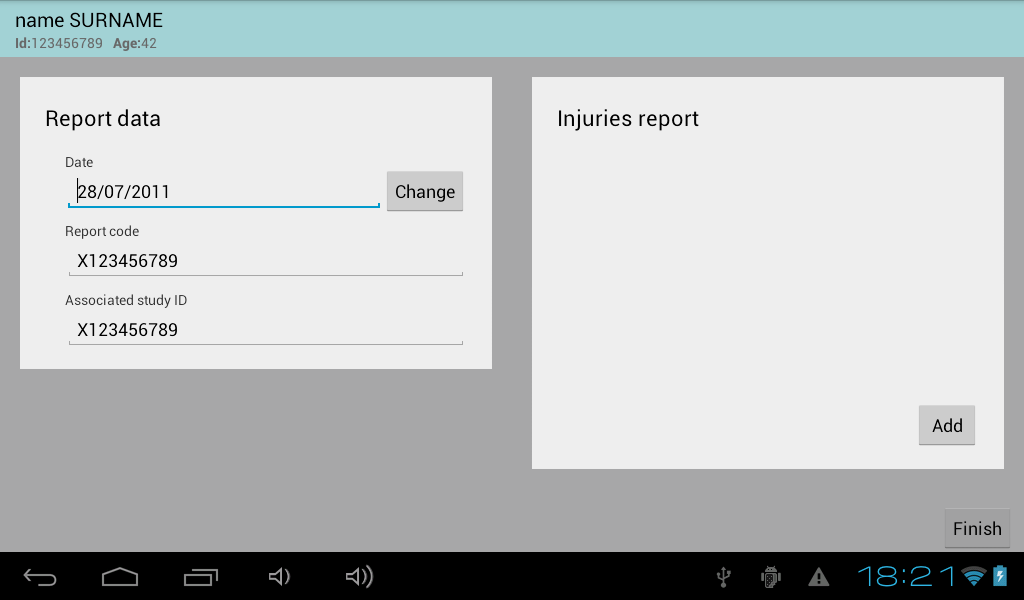
\includegraphics[scale=0.4]{./imgs/prototipo/landing.png}
\caption{Prototipo: Inicio de la aplicación.}
\label{fig:prototipo:inicio}
\end{figure}

\begin{figure}[ht]
\centering
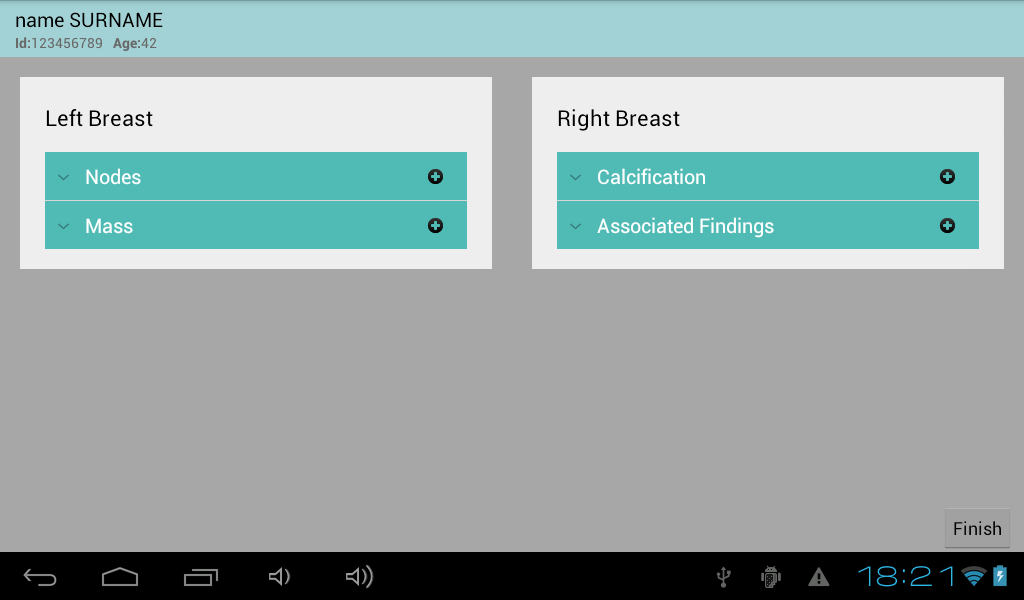
\includegraphics[scale=0.4]{./imgs/prototipo/close-tree.png}
\caption{Prototipo: Lista con las posibles lesiones de una mamografía.}
\label{fig:prototipo:tree}
\end{figure}

\begin{figure}[ht]
    \centering
    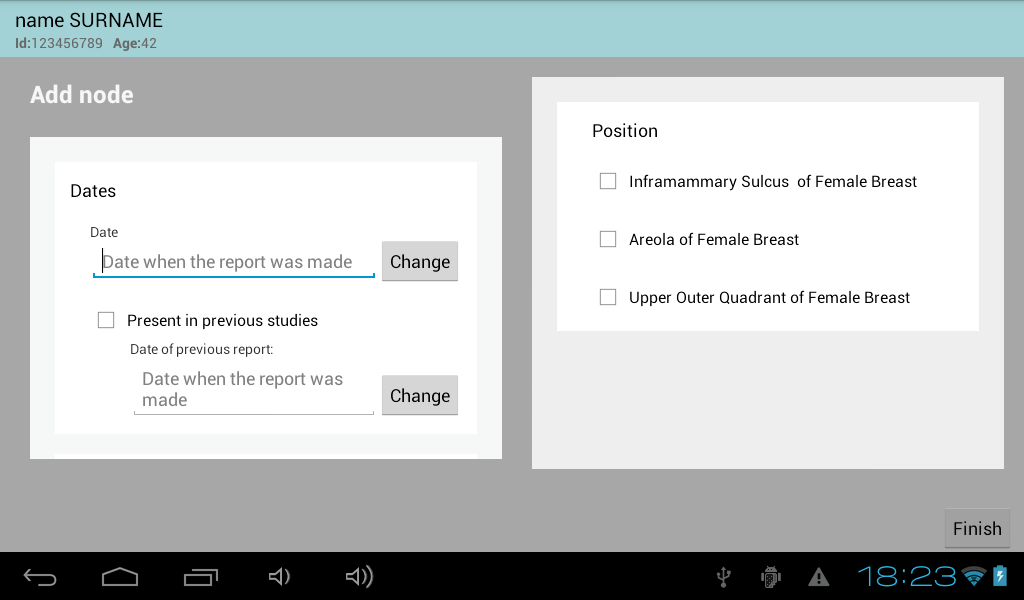
\includegraphics[scale=0.4]{./imgs/prototipo/addnode.png}
    \caption{Prototipo:Añadir un nódulo a la mama izquierda.}
    \label{fig:prototipo:add}
\end{figure}%


\begin{figure}[ht]
\centering
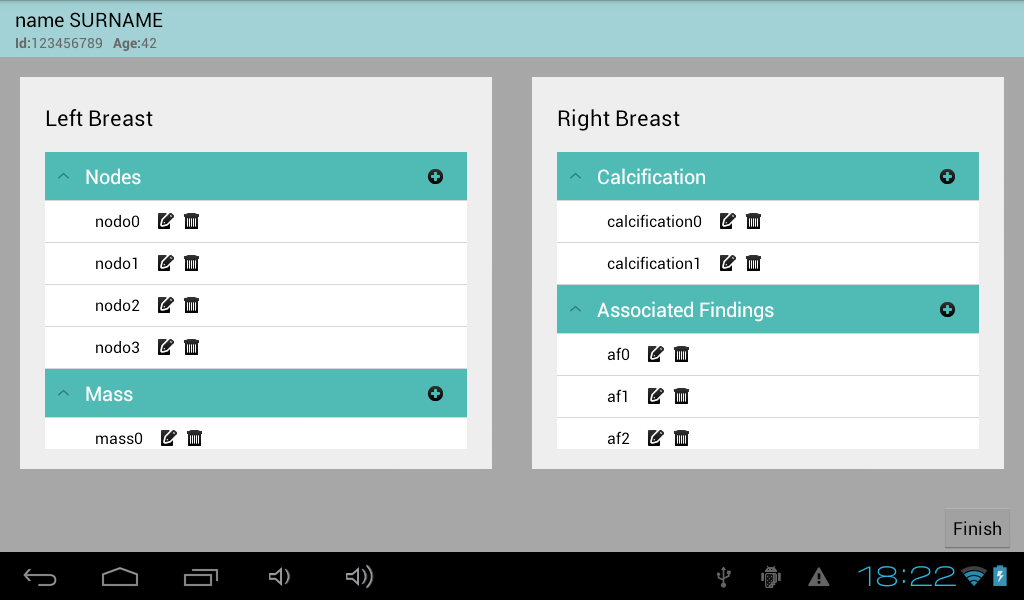
\includegraphics[scale=0.4]{./imgs/prototipo/open-tree.png}
\caption{Prototipo: Lista desplegada con las lesiones de una mamografía.}
\label{fig:prototipo:treenodes}
\end{figure}


\begin{figure}[ht]
    \centering
    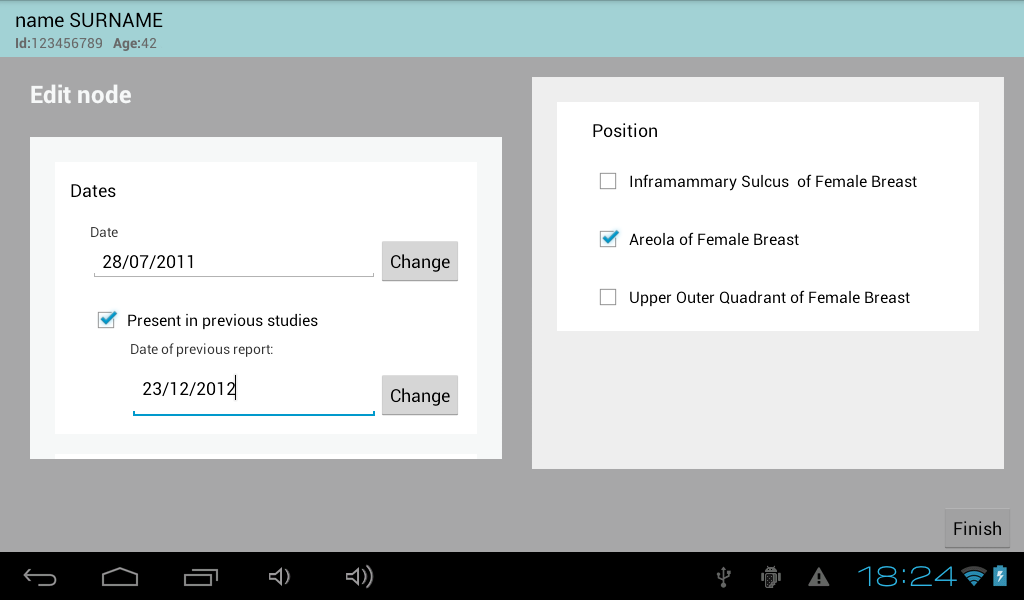
\includegraphics[scale=0.4]{./imgs/prototipo/editnode.png}
    \caption{Prototipo: Editar un nódulo a la mama izquierda.}
    \label{fig:prototipo:edit}
\end{figure}

Este prototipo nos ha servido para validar el diseño que hemos creado. Como hemos descrito a lo largo de esta etapa de desarrollo tanto el diseño como las interacciones con el usuario varían para adaptarse a sus necesidades reales.\par 




